%%%%%%%%%%%%%%%%%%%%%%%%%%%%%%%%%%%%%%%%%
\documentclass{article} % 'openany' here removes the gap page between days, erase it to restore this gap; 'oneside' can also be added to remove the shift that odd pages have to the right for easier reading

\usepackage[margin=1.00in]{geometry}

\usepackage[
  backref=page,
  pdfpagelabels=true,
  plainpages=false,
  colorlinks=true,
  bookmarks=true,
  pdfview=FitB]{hyperref} % Required for the hyperlinks within the PDF

\usepackage{booktabs} % Required for the top and bottom rules in the table
\usepackage{float} % Required for specifying the exact location of a figure or table
\usepackage{graphicx} % Required for including images2
\usepackage{lipsum} % Used for inserting dummy 'Lorem ipsum' text into the template
\usepackage{subfigure}
\newcommand{\HRule}{\rule{\linewidth}{0.5mm}} % Command to make the lines in the title page
\setlength\parindent{0pt} % Removes all indentation from paragraphs



%---------------------------------------------------------------------------------------
%%% TO ADD MATLAB FILES %%%%%
\usepackage{listings}
\lstset{basicstyle=\ttfamily\footnotesize,breaklines=true}

\usepackage{courier}
\lstset{basicstyle=\footnotesize\ttfamily,breaklines=true}
\lstset{framextopmargin=7pt,frame={topline}}


\usepackage{color} %red, green, blue, yellow, cyan, magenta, black, white
\definecolor{mygreen}{RGB}{28,172,0} % color values Red, Green, Blue
\definecolor{mylilas}{RGB}{170,55,241}
%%%%%%%%%%%%%%%%%%%%%%%%%%%%%

\graphicspath{{../Figures/}} % setting graphics path

\begin{document}

% ---------------- TO ADD MATLAB FILES --------
\lstset{language=Matlab,%
    %basicstyle=\color{red},
    breaklines=true,%
    morekeywords={matlab2tikz},
    keywordstyle=\color{blue},%
    morekeywords=[2]{1}, keywordstyle=[2]{\color{black}},
    identifierstyle=\color{black},%
    stringstyle=\color{mylilas},
    commentstyle=\color{mygreen},%
    showstringspaces=false,%without this there will be a symbol in the places where there is a space
    numbers=left,%
    numberstyle={\tiny \color{black}},% size of the numbers
    numbersep=9pt, % this defines how far the numbers are from the text
    emph=[1]{for,end,break},emphstyle=[1]\color{red}, %some words to emphasise
    %emph=[2]{word1,word2}, emphstyle=[2]{style},
}
%%%%%%%%%%%%%%%%%%%%%%%%%%%%%%%%%%%%%%%%%%%%%%%

%----------------------------------------------------------------------------------------
%	TITLE PAGE
%----------------------------------------------------------------------------------------

%\frontmatter % Use Roman numerals for page numbers
\title{
\begin{center}
\HRule \\[0.4cm]
{\Huge \bfseries Experiment-02: Potentiometer Data Acquisition and Pendulum Calibration \\[0.5cm] \Large ME-330}\\[0.4cm] % Degree
\HRule \\[1.5cm]
\end{center}
}
\author{\Huge Dr. Christopher Bitikofer \\ \\ \LARGE bitikofer@uidaho.edu \\[2cm]} % Your name and email address
\date{Fall 2024 Week-02} % Beginning date
\maketitle

\tableofcontents

\clearpage

\section{Learning objective}
This experiment provides students the opportunity to:

\begin{itemize}
\item Learn to use Matlab's data acquisition toolbox.
\item Create a simple program for data acquisition using Matlab and National Instrument’s myDAQ.
\item Become familiar with breadboards, digital power supply, wiring, digital multi-meters, and develop applied laboratory skills.
\item Calibrate a potentiometer-based angle measurement system and create a calibration plot.
\item Plot the time evolution (angle vs. time data) for a swinging motion of the pendulum system.
\end{itemize}

\section{Introduction}
In this experiment, you will connect a simple angle sensor (angular potentiometer) to the NI myDAQ data acquisition device and collect digital data using the Matlab data acquisition toolbox. First, you will collect data to create a calibration equation, then use the information from the calibration to convert the output voltage from the angular potentiometer to the pendulum angle. \\ \\

\large {\textbf{It is important that you read this entire document before the experiment. If you have questions about the procedure, instruction provided, or the code, please visit office hours to talk to me or the TAs before Thursday. }}

\section{Part-A: Creating Experiment Code}
\emph{Preparing data acquisition program using Matlab data acquisition toolbox}\\
The appendix of this document provides a Matlab program to use in this experiment. The main program sets the parameters for data acquisition. The "event listeners" lh1 and lh2 repeatedly call helper functions logData() and plotAndLogData(), which are responsible for capturing data to file and displaying it as it is acquired on a plot during experiments. 


\section{Part-B: Building the Potentiometer Circuit }
\emph{Connect an angular potentiometer to the NI My-DAQ using a breadboard}.
\begin{itemize}
\item Connect the potentiometer leads labeled “Power and Ground” to the 5 Volt reference signal and the reference ground from the power supply (Figure \ref{fig:fig02}).
\item Connect the NI MyDAQ to the angular potentiometer leads labeled “Signal and Ground”. The red wire should connect to AI0+ and the black wire to AI0- as shown (Figure  \ref{fig:fig02}).
%\begin{itemize}
%\item The AI0+(Analog Input 0 positive) and AI0-(Analog Input 0 negative) screw terminals are ``differential'' inputs in that both the ground voltage and the measured voltage are input and then the DAQ determines the difference between them. The ``ground input'' in the DAQ should not be connected to ground on the breadboard.
%\item When connecting wires to the screw terminals, put the wire above the metal tab and then turn the screw to the right. This will bring the metal tab up and tighten the wire in place.
%\item Make sure to check connections if the wires are engaged to the screw terminals by wiggling/tugging the wires.
%\end{itemize}
\end{itemize}
%\begin{figure}%
%\centering
%\subfigure[Sample breadboard connection.]{%
%\label{fig:fig01A}%
%\includegraphics[width=3.0in]{Fig01new.png}}%
%\qquad
%\subfigure[Sample breadboard connection along with DMM.]{%
%\label{fig:fig01B}%
%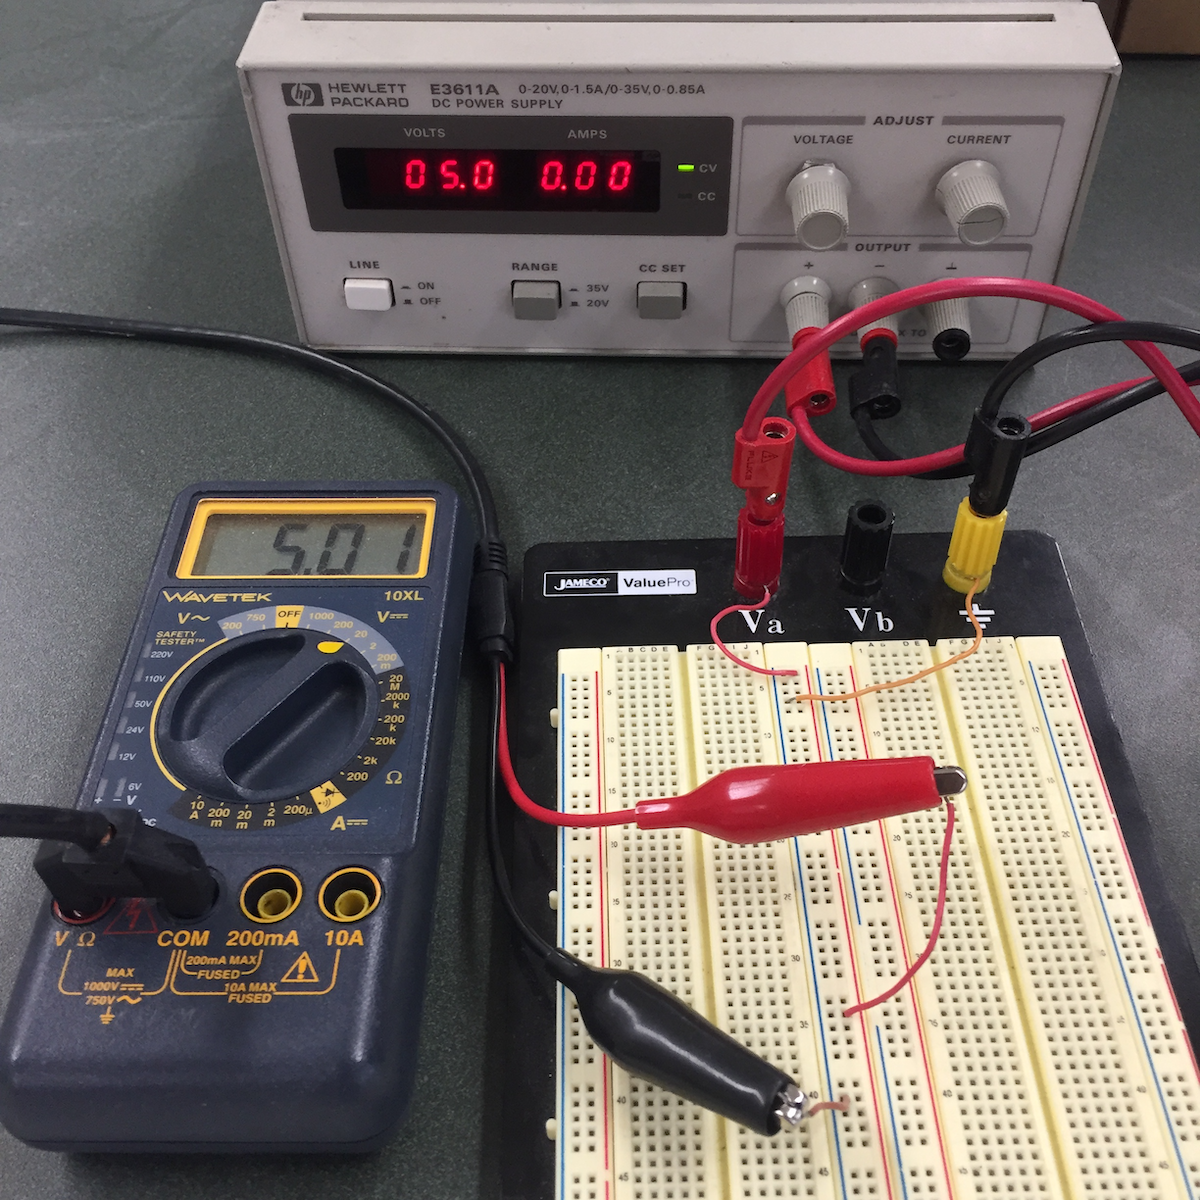
\includegraphics[width=3.0in]{Fig02.png}}%
%\caption{Bread board connection for experiment 2.}
%\end{figure}

\begin{figure}[!ht]
\centering
\includegraphics[width=3.00in]{Figures/Fig01new.jpg}
\caption{Connection to NI-DAQ system for experiment-2.}
\label{fig:fig02}
\end{figure}

\newpage
\section{Part-C: Testing code and circuit}
\emph{Run the acquisition program and test the circuit connections}.
\begin{itemize}
\item Verify your circuit with the TAs
\item Once your circuit is verified, run the tester acquisition program (see appendix \ref{app:testingCode}).
\item Rotate the angular potentiometer and verify the results. The display should change with the movement of the pendulum.
\item Keep in mind that DAQ system takes a while to initialize. There may be a slight delay before data acquisition starts.
\end{itemize}

\section{Part-D: Perform Calibration}
\emph{Create a calibration equation for the potentiometer to map output from volts to pendulum angle.}
\begin{itemize}
\item Determine a repeatable method for measuring the pendulum's angular position using either the supplied protractor (or an application on your phone, e.g., bubble level).
\item You will use the Matlab code in appendix \ref{app:calibCode} to perform the calibration.  
\item At each of 10 (or more) angles, ranging from $\pm$90 degrees, collect the voltage at a sampling rate of 20 Hz for 5 seconds. Save each of these files with the following name Ang\_(p/m)XXDeg.dat where xx represent angle and p/m represent plus or minus sign. For instance, the calibration file for $-45^o$ will be saved as ``Ang\_m45Deg.dat'' and  the calibration file for $+60^o$ will be saved as ``Ang\_p60Deg.dat''.
\begin{itemize}
	\item Make sure to document the pendulum angle for each recording \bf{in degrees}.
	\item {\bf The zero degree angle is when the pendulum is straight down.}
\end{itemize}
\item Create a table in log book similar to the table \ref{tab:Table01}. You will use the values in the table for calibration.
\item Plot the data collected calibration data using Matlab. The x-axis should be the recorded average voltages and the y-axis should be the angle in degrees. Be sure to properly annotate your plot. \textbf{Use the instruction from lab-01}
\item Use Matlab’s polyfit tool to determine a linear fit to the calibration data. This is your calibration equation. \textbf {Make sure to save your data in case you need to repeat any analysis}.
\item Record the norm of the residuals from the linear regression provided by Matlab’s polyfit function. Use this to calculate the standard error of the fit ($s_{yx}$).
\item See the sample code in appendix to generate the calibration plot \ref{app:genCalib}.
\item You need to modify `x' and `y' variables values in the code based on your calibration data.
\item Make sure to save the calibration file with at least 600 dpi resolution.
\end{itemize}

\begin{table}[!ht]
\centering
\caption{Sample calibration data for experiment 2.}
\begin{tabular}{c c}
\toprule
Pendulum angle (degree) & Average output voltage (v) \\ \hline
-90$^\circ$ & 1.21\\
-70$^\circ$ & 1.43\\
-50$^\circ$ & 1.65 \\
-30$^\circ$ & 2.00\\
-10$^\circ$ & 2.31\\
0$^\circ$  & 2.50\\
10$^\circ$ & 2.55\\
30$^\circ$ & 2.82\\
50$^\circ$ & 3.20\\
70$^\circ$ & 3.51\\
90$^\circ$ & 3.74\\
\bottomrule
\end{tabular}
\label{tab:Table01}
\end{table}

\section{Part-E: Acquire Pendulum Swing Data}
\emph{Add the calibration equation to the acquisition program to display the pendulum angle in degrees during the data acquisition process. }
\begin{itemize}
\item Update the slope and intercept values to reflect your calibration results in the provided Matlab program (Appendix \ref{app:acqCode}).
\item Show your program and results to the TAs to verify your program.
\item Change the acquisition time in the Matlab program to 15 seconds at a sampling rate of 200 Hz.
\item You will need to save the data for this part. Change the output file name to ``AngVsTime.dat''
\item Make sure your program is modified to acquire and store data to file.
\item Run your Matlab program to store the time and angle data.
\item Soon after you execute the program and acquisition initiates, release the pendulum from a horizontal position.
\item If your program is implemented correctly, it should display the angle (in degrees from your calibration equation) vs. time.
\item Confirm the file is stored correctly.
\item Open the stored data file and determine the period, $T_d$, of the response oscillations and the corresponding frequency, $\omega_d$.
\end{itemize}


\section{Part-F: Lab space clean up}
Return lab space to prior condition
\begin{itemize}
\item Remove all breadboard wires and place them back in the wire kit in an organized fashion.
\item Remove the pendulum wires from the breadboard and set aside.
\item Log off the computer.
\item {\bf Do this for every lab!}
\end{itemize}


\section{General Instruction}
\begin{itemize}
\item Make sure to name the files your FirstName\_ LastName\_ QuestionNumber, use the format provided in the sample Matlab code. Make sure the submitted figure is titled with your name. Include the apostrophe!
\item Make sure to submit your post-lab assignment on the Canvas website.
\item Here are some details to help.
\begin{itemize}
\item Plot the experimental data using red circles with MarkerSize 8. Experimental data points should always be plotted using markers without lines connecting the points.
\item Plot curve from theory (or curve fit line) using a solid colored line with LineWidth 2.
\item  Set the x and y-axis limits for each figure.
\item Make sure the major grid lines are visible.
\item All plot text should be in Times font. You will need to specify this for the title, labels, and legends. The axis labels and numbers should be in 10-point font.
\item The title should be in 10-point font.
\item Make sure to add the legend. Keep in mind that legend should not hide the plotted data.
\item For full credit, make sure that your submitted files look similar to the sample figures shown in the document.
\item If in doubt, make sure to request help from the TAs.
\end{itemize}
\end{itemize}

\clearpage

\clearpage
\section{Post lab (50 points)}
\textbf {Postlabs are due Friday at 5 pm.} For this experiment, submit the following items on Canvas for your post-laboratory assessment.
\begin{enumerate}
\item \textbf{Calibration plot}. Submit a calibration plot showing the raw data points as markers and the calibration curve as a line. 
\begin{itemize}
\item The plot should be 6.5” wide and 4.5" tall. 
\item Properly annotate your plots: axis labels, titles, legend, etc. Make sure to include units.
\item Using the text command in Matlab, place the equations or numbers listed below on the plot. Use Greek symbols where appropriate.  Make sure to include units. 
\begin{itemize}
    \item	The calibration equation on the plot with 4 decimals places for each number.
    \item	The norm of the residuals of your linear regression.
    \item	The standard error of the fit for your calibration equation.
\end{itemize}
\end{itemize}
\item \textbf{Pendulum Swing Plot.}  Submit a time series plot showing the trajectory of your pendulum swinging from a horizontal starting position. 
\begin{itemize}
    \item The plot should be 6.5” wide and 4.5" tall. 
    \item Make sure to properly annotate your plots: axis labels, titles, legend, etc.
    \item Using the text command in Matlab, place the equations or numbers listed below on the plot. Use Greek symbols where appropriate.
    \begin{itemize}
        \item	The period of the oscillations, $T_d$.
        \item The frequency of the oscillations, $\omega_d$.
    \end{itemize}
\end{itemize}
  

\item Answer all questions in the post-lab assessment on Canvas.
\end{enumerate}

\clearpage


%\section{Appendix}
%\subsection{Matlab program to test the circuit}
%\label{app:testingCode}
%\lstinputlisting{../Code/Expt02_Test.m}

%\clearpage

%\subsection{Matlab program to acquire data for calibration}
%\label{app:calibCode}
%\lstinputlisting{../Code/Expt02_Calibration.m}

%\clearpage
%\subsection{Matlab program to generate calibration plot}
%\label{app:genCalib}
%\lstinputlisting{../Code/Expt02_Calibration_plotting.m}

%\clearpage
%\subsection{Matlab program to acquire data}
%\label{app:acqCode}
%\lstinputlisting{../Code/Expt02_Data_aquisition.m}
%-----------------------------------------

\end{document} 